\documentclass[fleqn, 12pt]{article}\usepackage[]{graphicx}\usepackage[]{color}
% maxwidth is the original width if it is less than linewidth
% otherwise use linewidth (to make sure the graphics do not exceed the margin)
\makeatletter
\def\maxwidth{ %
  \ifdim\Gin@nat@width>\linewidth
    \linewidth
  \else
    \Gin@nat@width
  \fi
}
\makeatother

\definecolor{fgcolor}{rgb}{0.345, 0.345, 0.345}
\newcommand{\hlnum}[1]{\textcolor[rgb]{0.686,0.059,0.569}{#1}}%
\newcommand{\hlstr}[1]{\textcolor[rgb]{0.192,0.494,0.8}{#1}}%
\newcommand{\hlcom}[1]{\textcolor[rgb]{0.678,0.584,0.686}{\textit{#1}}}%
\newcommand{\hlopt}[1]{\textcolor[rgb]{0,0,0}{#1}}%
\newcommand{\hlstd}[1]{\textcolor[rgb]{0.345,0.345,0.345}{#1}}%
\newcommand{\hlkwa}[1]{\textcolor[rgb]{0.161,0.373,0.58}{\textbf{#1}}}%
\newcommand{\hlkwb}[1]{\textcolor[rgb]{0.69,0.353,0.396}{#1}}%
\newcommand{\hlkwc}[1]{\textcolor[rgb]{0.333,0.667,0.333}{#1}}%
\newcommand{\hlkwd}[1]{\textcolor[rgb]{0.737,0.353,0.396}{\textbf{#1}}}%
\let\hlipl\hlkwb

\usepackage{framed}
\makeatletter
\newenvironment{kframe}{%
 \def\at@end@of@kframe{}%
 \ifinner\ifhmode%
  \def\at@end@of@kframe{\end{minipage}}%
  \begin{minipage}{\columnwidth}%
 \fi\fi%
 \def\FrameCommand##1{\hskip\@totalleftmargin \hskip-\fboxsep
 \colorbox{shadecolor}{##1}\hskip-\fboxsep
     % There is no \\@totalrightmargin, so:
     \hskip-\linewidth \hskip-\@totalleftmargin \hskip\columnwidth}%
 \MakeFramed {\advance\hsize-\width
   \@totalleftmargin\z@ \linewidth\hsize
   \@setminipage}}%
 {\par\unskip\endMakeFramed%
 \at@end@of@kframe}
\makeatother

\definecolor{shadecolor}{rgb}{.97, .97, .97}
\definecolor{messagecolor}{rgb}{0, 0, 0}
\definecolor{warningcolor}{rgb}{1, 0, 1}
\definecolor{errorcolor}{rgb}{1, 0, 0}
\newenvironment{knitrout}{}{} % an empty environment to be redefined in TeX

\usepackage{alltt}
\usepackage{amsmath}
\usepackage{amssymb}
\usepackage{geometry}
\usepackage{graphicx}
\usepackage{bm}
\usepackage{url}
\usepackage{enumerate}
\usepackage{fullpage}
\IfFileExists{upquote.sty}{\usepackage{upquote}}{}
\begin{document}
\setlength\parindent{0pt}

\Large
\textbf{Lab 6: Introduction to the Bootstrap}\\
\large
\textbf{STAT 630, Fall 2020}\\
\normalsize

The bootstrap is a data based simulation method for statistical inference that can be used to compute standard errors and construct confidence intervals.  The term ``bootstrap" derives from the phrase ``to pull oneself up by one's bootstrap."  It is a useful technique for constructing confidence intervals when there is no analytic (mathematical) formula to work with, or if the assumption for using a formula are not well satisfied.\\  

\textbf{Bootstrap Algorithm}:
\begin{enumerate}
\item Let $x_1, x_2, \cdots, x_n$ be a sample of size $n$; and $\hat{\theta}$ a statistic computed using this sample (e.g., mean, median, trimmed mean, standard deviation, etc.)
\item Take a sample with replacement of size $n$ from the original sample.  Call this the \textbf{bootstrap sample}.
\item Recompute the statistic of interest using the bootstrap sample.  Call this the \textbf{bootstrap replicate} of the statistic, denoted by $\theta^*$.
\item Repeat steps 2 and 3 $B$ times to generate $B$ bootstrap replicates of the statistic: $\theta_1^*, \theta_2^*, \cdots, \theta_B^*$.  The distribution of the bootstrap replicates is called the \textbf{bootstrap distribution}.\\
\end{enumerate}

\textbf{Sampling with replacement} means that an observation can occur more than once in the bootstrap sample.  For example, if $x_1, x_2, x_3, x_4, x_5$ is a sample of size $n=5$, then $x_1, x_2, x_3, x_3, x_5$ is a possible bootstrap sample.  Or think of it this way: write the numbers 1 though 100 on tickets and place in a hat, then each time you draw a random number from that hat throw it back in.\\ 

\textbf{Bootstrap Standard Error}:  A bootstrap estimate of the standard error of a statistic can be computed as the the standard deviation of the bootstrap replicates of the statistic, i.e., the standard deviation of $\theta_1^*, \theta_2^*, \cdots, \theta_B^*$.\\

\textbf{Bootstrap Percentile Confidence Interval}:  A 95\% bootstrap confidence interval for a parameter $\theta$ can be computed as the 0.025 and 0.975 quantiles of the bootstrap replicates of the statistic, i.e., the 0.025 and 0.975 quantiles of $\theta_1^*, \theta_2^*, \cdots, \theta_B^*$.  We can use the \texttt{quantile()} function in R to do this.\\   
\clearpage

\textbf{Remarks}
\begin{itemize}
\item The main idea behind the bootstrap procedure is that if the sample is representative of the population, then the bootstrap distribution should approximate the shape and spread of the sampling distribution of a statistic.  So we can use the bootstrap method to learn something about the sampling distribution of a statistic, and how close that statistic is to the true value (population parameter).
\item The bootstrap distribution should be centered around the statistic $\hat{\theta}$ (not the parameter $\theta$).  So the bootstrap is not useful for getting a more accurate estimate of $\theta$, but rather for characterizing the variability (standard error) of that statistic.\\ 
\end{itemize}

\textbf{Example}\\
For this example, we use a data set containing arsenic concentration in 271 wells in Bangladesh.  Arsenic is a naturally occurring element in the groundwater in Bangladesh; since much of this water is used for drinking in rural areas, arsenic poisoning is a major health problem.  To access the data set first install the \texttt{resampledata} package, and then use \texttt{library()} to load the package into your workspace.

\begin{knitrout}
\definecolor{shadecolor}{rgb}{0.969, 0.969, 0.969}\color{fgcolor}\begin{kframe}
\begin{alltt}
\hlkwd{library}\hlstd{(resampledata)}
\end{alltt}
\end{kframe}
\end{knitrout}

First, let's look at some descriptive statistics for Arsenic.  Note that the arsenic measurements are in micrograms per liter ($\mu$g/L).

\begin{knitrout}
\definecolor{shadecolor}{rgb}{0.969, 0.969, 0.969}\color{fgcolor}\begin{kframe}
\begin{alltt}
\hlstd{Arsenic} \hlkwb{<-} \hlstd{Bangladesh}\hlopt{$}\hlstd{Arsenic}
\hlkwd{summary}\hlstd{(Arsenic)}
\end{alltt}
\begin{verbatim}
##    Min. 1st Qu.  Median    Mean 3rd Qu.    Max. 
##     0.5     6.0    22.0   125.3   109.0  2400.0
\end{verbatim}
\begin{alltt}
\hlkwd{sd}\hlstd{(Arsenic)}
\end{alltt}
\begin{verbatim}
## [1] 297.9755
\end{verbatim}
\begin{alltt}
\hlkwd{par}\hlstd{(}\hlkwc{mfrow}\hlstd{=}\hlkwd{c}\hlstd{(}\hlnum{1}\hlstd{,}\hlnum{2}\hlstd{))}
\hlkwd{hist}\hlstd{(Arsenic)}
\hlkwd{qqnorm}\hlstd{(Arsenic)}
\hlkwd{qqline}\hlstd{(Arsenic)}
\end{alltt}
\end{kframe}
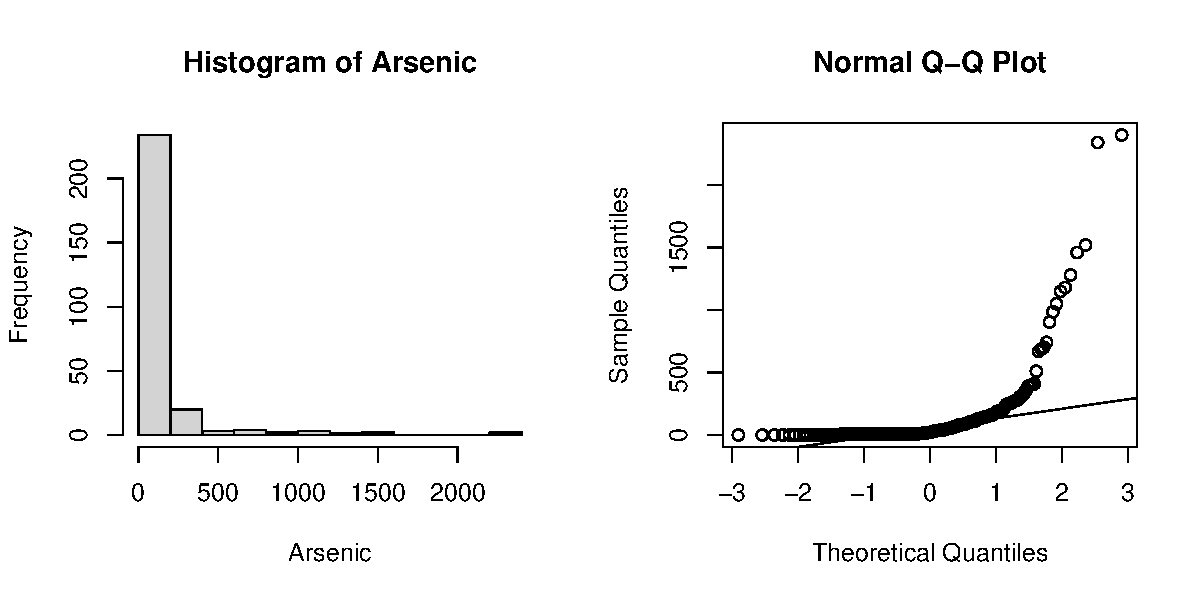
\includegraphics[width=\maxwidth]{figure/unnamed-chunk-2-1} 

\end{knitrout}

We see that the shape of the histogram of the sample is heavily skewed to the right.\\

Next, draw 5000 bootstrap samples of arsenic.  Compute the mean of each bootstrap sample to get 5000 bootstrap replicates.  Then use the 5000 bootstrap replicates to compute the bootstrap standard error and 95\% confidence interval.

\begin{knitrout}
\definecolor{shadecolor}{rgb}{0.969, 0.969, 0.969}\color{fgcolor}\begin{kframe}
\begin{alltt}
\hlkwd{set.seed}\hlstd{(}\hlnum{9999}\hlstd{)}
\hlstd{n} \hlkwb{<-} \hlkwd{length}\hlstd{(Arsenic); n}
\end{alltt}
\begin{verbatim}
## [1] 271
\end{verbatim}
\begin{alltt}
\hlstd{replicates} \hlkwb{<-} \hlkwd{rep}\hlstd{(}\hlnum{0}\hlstd{,} \hlnum{5000}\hlstd{)}
\hlkwa{for}\hlstd{(i} \hlkwa{in} \hlnum{1}\hlopt{:}\hlnum{5000}\hlstd{) \{}
  \hlstd{boot_samp} \hlkwb{<-} \hlkwd{sample}\hlstd{(Arsenic,} \hlkwc{size} \hlstd{= n,} \hlkwc{replace} \hlstd{=} \hlnum{TRUE}\hlstd{)}
  \hlstd{replicates[i]} \hlkwb{<-} \hlkwd{mean}\hlstd{(boot_samp)}
\hlstd{\}}

\hlcom{# bootstrap distribution}
\hlkwd{par}\hlstd{(}\hlkwc{mfrow}\hlstd{=}\hlkwd{c}\hlstd{(}\hlnum{1}\hlstd{,}\hlnum{2}\hlstd{))}
\hlkwd{hist}\hlstd{(replicates,} \hlkwc{xlab}\hlstd{=}\hlstr{"Replicates of sample mean"}\hlstd{,} \hlkwc{main}\hlstd{=}\hlstr{''}\hlstd{)}
\hlkwd{abline}\hlstd{(}\hlkwc{v}\hlstd{=}\hlkwd{mean}\hlstd{(Arsenic),} \hlkwc{col}\hlstd{=}\hlstr{"cyan"}\hlstd{,} \hlkwc{lwd}\hlstd{=}\hlnum{2}\hlstd{)}
\hlkwd{qqnorm}\hlstd{(replicates)}
\hlkwd{qqline}\hlstd{(replicates)}
\end{alltt}
\end{kframe}
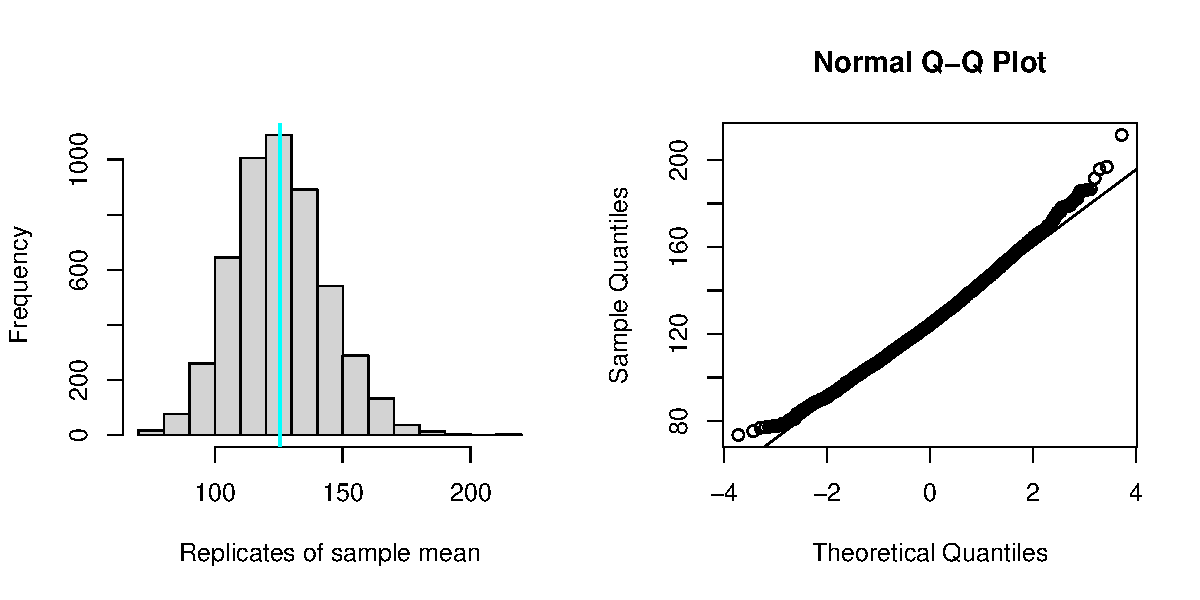
\includegraphics[width=\maxwidth]{figure/unnamed-chunk-3-1} 
\begin{kframe}\begin{alltt}
\hlcom{# bootstrap standard error}
\hlkwd{sd}\hlstd{(replicates)}
\end{alltt}
\begin{verbatim}
## [1] 18.14656
\end{verbatim}
\begin{alltt}
\hlcom{# 95% bootstrap CI}
\hlkwd{quantile}\hlstd{(replicates,} \hlkwd{c}\hlstd{(}\hlnum{0.025}\hlstd{,} \hlnum{0.975}\hlstd{))}
\end{alltt}
\begin{verbatim}
##      2.5%     97.5% 
##  91.89089 162.95601
\end{verbatim}
\end{kframe}
\end{knitrout}



We are 95\% confident that the true mean arsenic level is between 91.89 and 162.96 micrograms per liter.  We can compare this to a traditional confidence interval for the mean calculated with a $z$-critical value.  Even though the population distribution is heavily skewed, the sample size $n=271$ is perhaps large enough so that the CLT provides justification.  

\begin{knitrout}
\definecolor{shadecolor}{rgb}{0.969, 0.969, 0.969}\color{fgcolor}\begin{kframe}
\begin{alltt}
\hlstd{ci_lower} \hlkwb{<-} \hlkwd{mean}\hlstd{(Arsenic)} \hlopt{-} \hlnum{1.96} \hlopt{*} \hlkwd{sd}\hlstd{(Arsenic)} \hlopt{/} \hlkwd{sqrt}\hlstd{(n)}
\hlstd{ci_upper} \hlkwb{<-} \hlkwd{mean}\hlstd{(Arsenic)} \hlopt{+} \hlnum{1.96} \hlopt{*} \hlkwd{sd}\hlstd{(Arsenic)} \hlopt{/} \hlkwd{sqrt}\hlstd{(n)}
\hlkwd{round}\hlstd{(}\hlkwd{c}\hlstd{(ci_lower, ci_upper),} \hlnum{2}\hlstd{)}
\end{alltt}
\begin{verbatim}
## [1]  89.84 160.80
\end{verbatim}
\end{kframe}
\end{knitrout}

Indeed, we see that the endpoints of 95\% bootstrap and $z$-confidence intervals are close.
\clearpage

A major motivation for the bootstrap is that it can be used with wide variety of statistics (means, medians, trimmed means, standard deviations, correlation coefficients).  The bootstrap is especially useful when there is no easy formula that we can work with to get a confidence interval.  For example, let's use the bootstrap to construct a confidence interval for the 25\% trimmed mean, also called the midmean; that is, the mean of the middle 50\% of observations.  

\begin{knitrout}
\definecolor{shadecolor}{rgb}{0.969, 0.969, 0.969}\color{fgcolor}\begin{kframe}
\begin{alltt}
\hlkwd{mean}\hlstd{(Arsenic,} \hlkwc{trim}\hlstd{=}\hlnum{0.25}\hlstd{)} \hlcom{# 25% trimmed mean}
\end{alltt}
\begin{verbatim}
## [1] 35.95985
\end{verbatim}
\begin{alltt}
\hlstd{replicates} \hlkwb{<-} \hlkwd{rep}\hlstd{(}\hlnum{0}\hlstd{,} \hlnum{5000}\hlstd{)}
\hlkwa{for}\hlstd{(i} \hlkwa{in} \hlnum{1}\hlopt{:}\hlnum{5000}\hlstd{) \{}
  \hlstd{boot_samp} \hlkwb{<-} \hlkwd{sample}\hlstd{(Arsenic,} \hlkwc{size} \hlstd{= n,} \hlkwc{replace} \hlstd{=} \hlnum{TRUE}\hlstd{)}
  \hlstd{replicates[i]} \hlkwb{<-} \hlkwd{mean}\hlstd{(boot_samp,} \hlkwc{trim} \hlstd{=} \hlnum{0.25}\hlstd{)}
\hlstd{\}}

\hlcom{# boostrap distribution}
\hlkwd{par}\hlstd{(}\hlkwc{mfrow}\hlstd{=}\hlkwd{c}\hlstd{(}\hlnum{1}\hlstd{,}\hlnum{2}\hlstd{))}
\hlkwd{hist}\hlstd{(replicates,} \hlkwc{xlab}\hlstd{=}\hlstr{"Replicates of the trimmed mean"}\hlstd{,} \hlkwc{main}\hlstd{=}\hlstr{''}\hlstd{)}
\hlkwd{abline}\hlstd{(}\hlkwc{v}\hlstd{=}\hlkwd{mean}\hlstd{(Arsenic,} \hlkwc{trim}\hlstd{=}\hlnum{0.25}\hlstd{),} \hlkwc{col}\hlstd{=}\hlstr{"cyan"}\hlstd{,} \hlkwc{lwd}\hlstd{=}\hlnum{2}\hlstd{)}
\hlkwd{qqnorm}\hlstd{(replicates)}
\hlkwd{qqline}\hlstd{(replicates)}
\end{alltt}
\end{kframe}
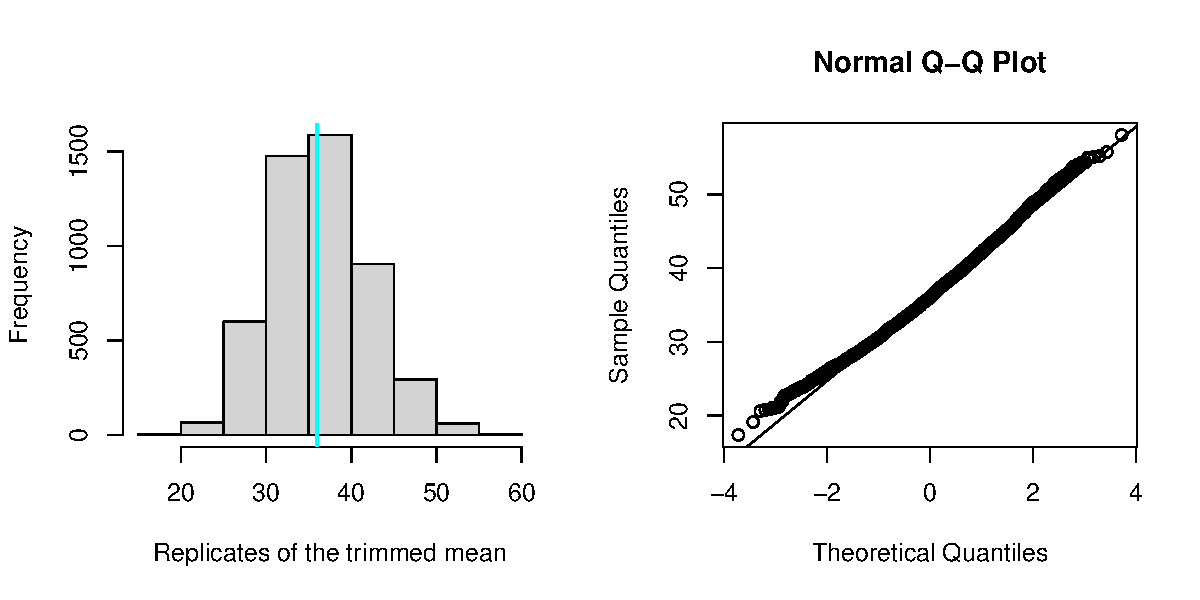
\includegraphics[width=\maxwidth]{figure/unnamed-chunk-6-1} 
\begin{kframe}\begin{alltt}
\hlcom{# bootstrap standard error}
\hlkwd{sd}\hlstd{(replicates)}
\end{alltt}
\begin{verbatim}
## [1] 5.717114
\end{verbatim}
\begin{alltt}
\hlcom{# 95% bootstrap CI}
\hlkwd{quantile}\hlstd{(replicates,} \hlkwd{c}\hlstd{(}\hlnum{0.025}\hlstd{,} \hlnum{0.975}\hlstd{))}
\end{alltt}
\begin{verbatim}
##     2.5%    97.5% 
## 26.26692 48.59909
\end{verbatim}
\end{kframe}
\end{knitrout}


We are 95\% confident that the true midmean for arsenic is between 26.27 and 48.6 micrograms per liter.  Notice that the bootstrap distribution for the trimmed mean has much smaller spread than the bootstrap distribution for the mean.  This is because the trimmed mean is more robust, and less sensitive to extreme values.\\

\textbf{Reference}:  Chihara, L., and Hesterberg T. Mathematical statistics with resampling and R, 2nd edition, Chapter 5. [Electronic version: \url{http://library.csueastbay.edu/home}]\\

\bigskip

\textbf{Practice Problem}. Using the arsenic data:
\begin{enumerate}[(a)]
\item Generate 5000 bootstrap replicates of the median.  Make a histogram of the 5000 replicates that you generated.
\item Compute the bootstrap standard error for the median.
\item Compute a 95\% bootstrap percentile confidence interval for the median.  Interpret the interval.
\end{enumerate}




\clearpage
\end{document}

